\documentclass[11pt]{article}
\usepackage{amsmath,amssymb,amsthm,mathtools,physics}
\usepackage[margin=1.0in]{geometry}
\usepackage{parskip}

\usepackage{graphics,graphicx,epstopdf}
\usepackage{float,tabularx,subcaption}

% Make \begin{bmatrix}\end{bmatrix} command accept alignment options like [rrr]
\makeatletter
\renewcommand*\env@matrix[1][*\c@MaxMatrixCols c]{%
\hskip -\arraycolsep
\let\@ifnextchar\new@ifnextchar
\array{#1}}
\makeatother
\begin{document}

\begin{figure}[H]
\centering
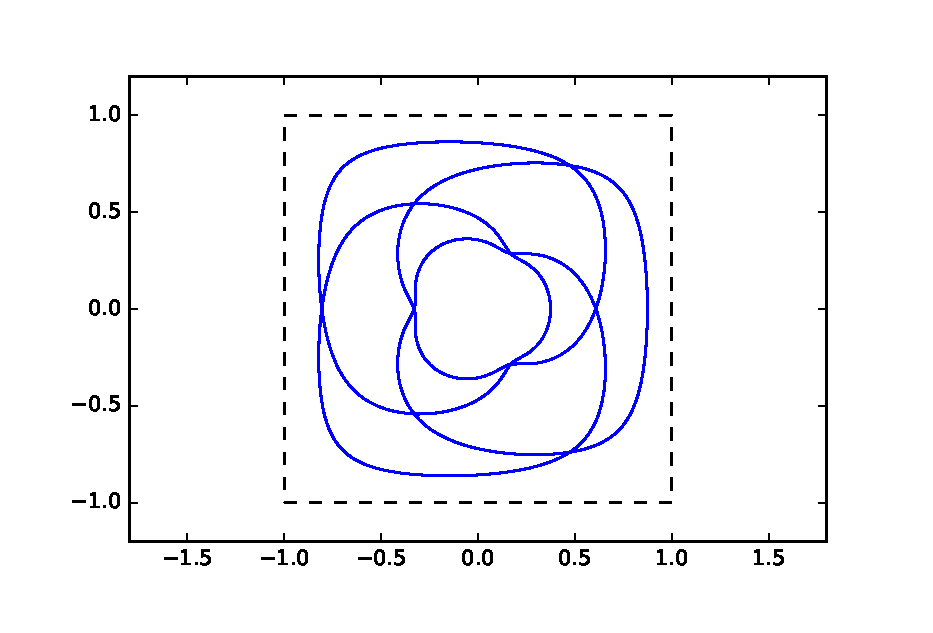
\includegraphics[width=\textwidth]{discToSquare_example1}
\caption{Plot generated by the Python library \textsc{matplotlib}.}
\end{figure}

\end{document}